First, we copy files \texttt{Controller.c}, \texttt{OwnVariables.c} and
\texttt{RenewControllerState.c} by opening each one, pressing \texttt{Ctrl+A}
and then \texttt{Ctrl+C} inside the editor.

We then navigate to the directory

\texttt{SOURCE\_RESIDENCE/Simulation Environment/ArduinoFiles/hybrid\_control.ino}

and double-click on \texttt{hybrid\_control.ino}. We scroll down until we locate
the parts where our code should be pasted. Upon finding them we immediately hit
\texttt{Ctrl+V}. Figure \ref{fig:20_1} shows a part of the process before
pasting the relevant copied file and figure \ref{fig:20_2} shows the outcome of
applying the action \texttt{Ctrl+V}.

\begin{figure}[H]
  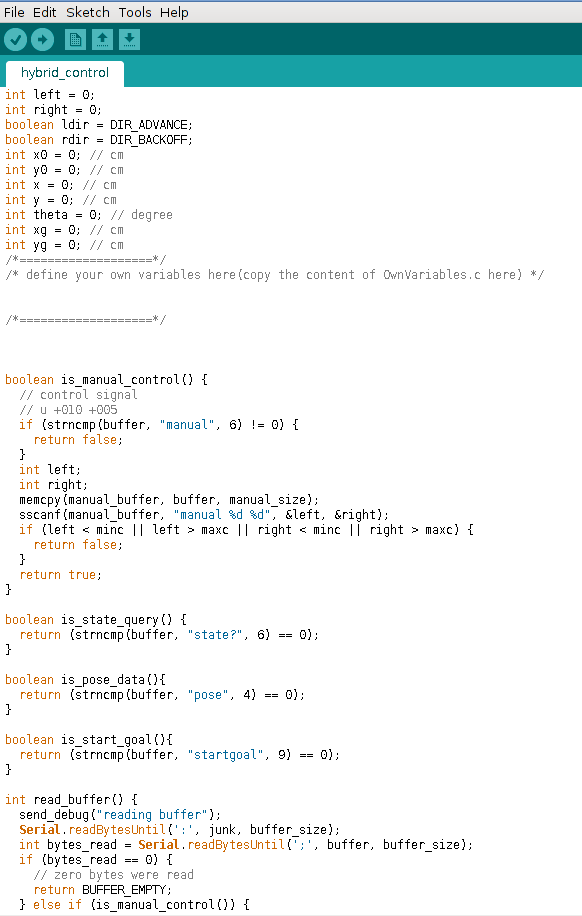
\includegraphics[scale=0.6]{./figures/task_20/1.png}
  \caption{\texttt{hybrid\_control.ino} before copying the contents of
    \texttt{OwnVariables.c} in it.}
  \label{fig:20_1}
\end{figure}

\begin{figure}[H]
  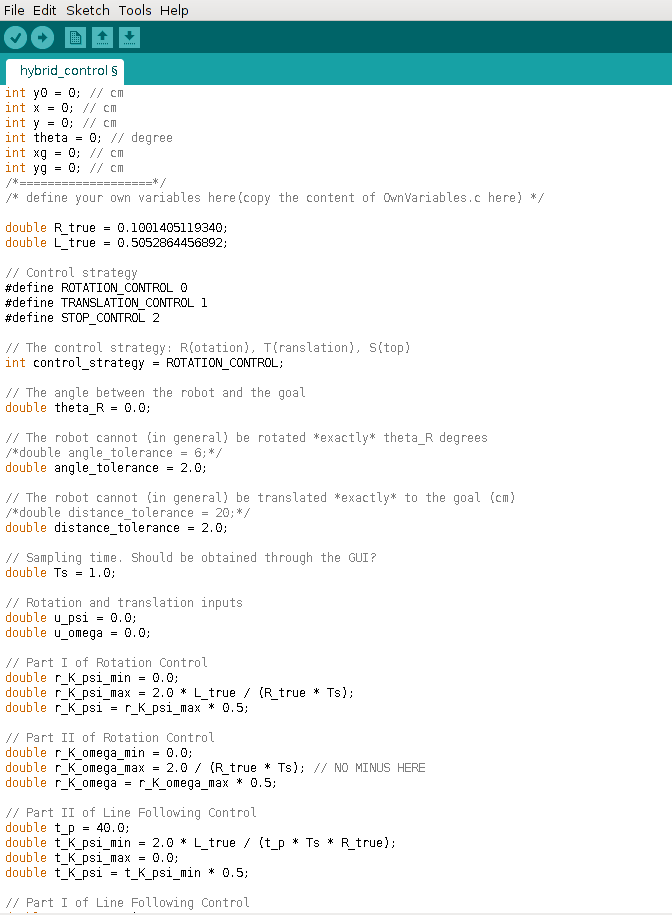
\includegraphics[scale=0.6]{./figures/task_20/2.png}
  \caption{\texttt{hybrid\_control.ino} after copying the contents of
    \texttt{OwnVariables.c} in it.}
  \label{fig:20_2}
\end{figure}

After the successful insertion of the contents of
the aforementioned files, we move the mouse to upper-left corner where we find
a tick symbol, illustrated in figure \ref{fig:20_3}. We then press it using the
left button of the mouse.

\begin{figure}[H]
  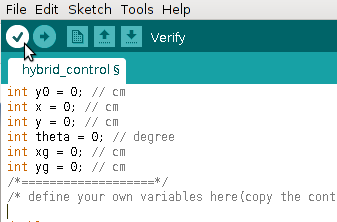
\includegraphics[scale=1]{./figures/task_20/3.png}
  \caption{After the injection of the contents of the three files we locate
    the tick symbol and click it}
  \label{fig:20_3}
\end{figure}
